\documentclass[12pt,a4paper]{article}

% -----------------------------
% Packages
% -----------------------------
\usepackage[utf8]{inputenc}    % UTF-8 encoding
\usepackage[T1]{fontenc}       % Better font encoding
\usepackage{lmodern}           % Better font rendering
\usepackage[scaled]{helvet}
\renewcommand{\familydefault}{\sfdefault}
\usepackage{geometry}          % Page margins
\usepackage{setspace}          % Line spacing
\usepackage{titlesec}          % Control section formatting
\usepackage{hyperref}          % Clickable links & TOC
\usepackage{graphicx}          % Images
\usepackage{fancyhdr}          % Headers & footers
\usepackage{listings}
\usepackage{xcolor}
\lstset{
  basicstyle=\ttfamily\small,  % Monospace for code
  backgroundcolor=\color{gray!10},
  frame=single,
  breaklines=true,
  showstringspaces=false,
  keywordstyle=\color{blue},
  commentstyle=\color{green!50!black},
  stringstyle=\color{red!70!black}
}
% Monospace font setup
\renewcommand{\ttdefault}{pcr}
% -----------------------------
% Page setup
% -----------------------------
\geometry{margin=1in}
\singlespacing
\setlength{\parskip}{0.5em}

% -----------------------------
% Section title formatting
% -----------------------------
\titleformat{\section}
  {\normalfont\Large\bfseries}{\thesection}{1em}{}
\titleformat{\subsection}
  {\normalfont\large\bfseries}{\thesubsection}{1em}{}

% -----------------------------
% Header & footer
% -----------------------------
\pagestyle{fancy}
\fancyhf{}
\lhead{ COAT (Certificate of analysis toolkit) Admin Guide }
\rhead{\thepage}

% -----------------------------
% Title info
% -----------------------------
\title{
  \Huge \textbf{
    COAT (Certificate of analysis toolkit) Admin Guide} \\
    \vspace{1em}
  \large ProteinSimple Toronto Operation department \\
  \large Author: Arvin Asgharian Rezaee
  }
 
\author{}
\date{\today}

% -----------------------------
% Document
% -----------------------------
\begin{document}

% Title page
\maketitle
\thispagestyle{empty}
\clearpage

% Table of contents
\tableofcontents
\clearpage

% -----------------------------
% Introduction
% -----------------------------
\section{Introduction}
COAT was first developed during summer of 2025 to automate and streamline the process of COA creation
for Maurice cartridges in the Toronto office. The purpose of this guide is to briefly cover the 
software architecture of the project, alongside instructions for maintaining and updating it.
\section{Getting Started}
We will first lightly touch upon compiling and deploying a project and releasing a new version.
\subsection{System Requirements}
At the time of creation of this document, the only supported OS for COAT is Windows 11 and Windows 10.
The released executable file only supports the mentioned Systems. Although the source code can be altered
to support other systems, there is currently no guarantee of compatibility. It is assumed that the
following software is installed and working correctly on your machine.
\begin{itemize}
  \item Git
  \item Winget
\end{itemize}

\subsection{Setup}
The source code for the project can be cloned with the following links: \newline
\textit{https://github.com/ProteinSimple/COA-Automation} \newline
To clone the project use the following command in your terminal
\begin{lstlisting}[language=bash]
cd ~
mkdir temp
cd temp
git clone https://github.com/ProteinSimple/COA-Automation.git .
\end{lstlisting}
The steps to install the program can be found in the GitHub webpage. Follow the steps to install the requirements
and run the project. 

\subsection{Deploying a new version}



\section{Action Guide}
The automation script that is the backend logic of COAT, is written
in python and has a CLI where you can provide the application with actions
you would like it to perform. This is in fact the exact method that the UI 
communicates with this script. The following is a list of possible actions
alongside a brief and non-technical explanation. The python file containing
the entry point to the program is listed below:
\begin{lstlisting}[language=bash]
<project path>/automation/src/main.py
\end{lstlisting}
To get comprehensive list of actions run the following
\begin{lstlisting}[language=bash]
> cd <project path>/automation/src
> python main.py --help
\end{lstlisting}
To get a description of an action alongside how to use it run it with "action-name --help"
so as an example:
\begin{lstlisting}[language=bash]
> python main.py check --help
\end{lstlisting}
Before diving into specifics of each action,  there are several common arguments
that are shared between all of the actions. Let's first have an overview of those:
\begin{itemize}
  \item -h, --help: Show help comments
  \item --run-mode: Set run mode of program (test or prod, default = prod)
  \item --verbose: By default the script outputs its results to the given output file.
                   with this option it will print it to stdout instead (default = False)
  \item --config: Path to the configuration file containing run information (default = ./config.yaml)
  \item --output: Output file used to showcase the result of the program
  \item --user: username for Saturn authentication
  \item --passkey: passkey for Saturn authentication 
\end{itemize}
\subsubsection{CLI response format}
The CLI program will have the following format for each output
\begin{lstlisting}[]
  <COMMAND_RESULT>
  <COMMAND_BODY>
\end{lstlisting}
Where the command result is a single bit passed as 1 or 0, indicating whether or not the command was successful.
The command body is either a JSON object that can be parsed to communicate information, or an empty string.
\subsubsection{Saturn Authentication}
To authenticate to Saturn (Mopho), the first time you run the program you must provide
the CLI with your username and passkey. For most actions this is  crucial. After initially providing the
credentials, COAT CLI will store the information and providing them again is not needed.
\subsection{Check Action}
Used to check if connection to Saturn is valid. Method of running is :
\begin{lstlisting}[]
  python main.py check
\end{lstlisting}
The command will check if using your current credentials you can access Saturn. This command does not produce a command body.

\subsection{Fetch Action}
Access Mopho QC dataset and Production dataset to retrieve cartridge information. It does so by joining the results
using the cartridge id.
\begin{lstlisting}[]
  python main.py fetch <start-date> <end-date>
\end{lstlisting}
The start and end dates must be in the format: YYYY-MM-DD (e.g., 2025-08-11). \newline
The command will check if using your current credentials you can access Saturn.
\subsubsection{Command body}
The command body is of the following format:
\begin{lstlisting}[language=python]
  {
    "values" : # list of cartridgeInfo,
    "start" : # production start date in YYYY-MM-DD,
    "end" : # production end date in YYYY-MM-DD
  }
\end{lstlisting}
Each of the cartridgeInfo is of the following format:
\begin{lstlisting}[language=python]
  {
    "id": # cartridge id,
    "build_date": # production date. format: MM/DD/YYYY,
    "build_time": # production time. format: HH:MM,
    "exp_date": # expiration date. format: MM/DD/YYYY,
    "class_name": # cartridge class name,
    "class_code": # cartridge class code,
    "batch_num": # Batch number,
    "qc_date": # QC run date. format: MM/DD/YYYY,
    "qc_time": # QC run time. format: HH:MM,
    "qc_analysis_date": # QC analysis date. format: MM/DD/YYYY,
    "qc_analysis_time": # QC analysis time. format: HH:MM,
    "qc_status": # result of most recent QC,
    "qc_user": # QC analyst name
  }
\end{lstlisting}
The start and the end date range are the production range which the cartridge is in.

\subsection{Config Action}
To edit and modify partial parts of the configuration file, the config action was developed to avoid any manual entry. The
following is the format of the command:
\begin{lstlisting}[language=bash]
  python main.py config <config_sub_action> ...
\end{lstlisting}
The sub action is one of the following : Add, Delete, List. We will go into in-depth description of these command in the next subsection.
\subsubsection{Command body}
The contents is a JSON style printout of the configuration YAML file. For further details of this configuration file see section 4. \newline
\newline
We will now give an overview of all Config sub actions:
\subsubsection{Config List}
The format of this sub command is:
\begin{lstlisting}[language=bash]
  python main.py config list
\end{lstlisting}
This command does not have any side effects and only purpose of it is to get the printout of the config file
\subsubsection{Config Add}
The format of this sub command is:
\begin{lstlisting}[language=bash]
  python main.py config add [--pdf PDF [PDF ...]] [--csv CSV [CSV ...]]
\end{lstlisting}
The pdf and the csv argument, is the output paths that are to be added to the config file. The output paths are stored as sets, meaning
duplicate paths are not allowed in either list. This action updates the configuration file at its location.
\subsubsection{Config Delete}
The format of this sub command is:
\begin{lstlisting}[language=bash]
  python main.py config delete [--pdf PDF [PDF ...]] [--csv CSV [CSV ...]]
\end{lstlisting}
This is similar to the previous sub-command, only that it deletes the given paths instead. 

\subsection{COA Action}
The purpose of this action is to produce COAs for the given cartridges. The format of this command is:
\begin{lstlisting}[language=bash]
  python main.py coa <ids ...> --start <start-date> --end <end-date>
\end{lstlisting}
\begin{itemize}
  \item ids: ids of the cartridges we want to create the COA for
  \item start: start date for the production range (production range is the date range where all the cartridges production date is in)
  \item end: end date for the production range
\end{itemize}
This action uses the information on the config file, to retrieve the template file and information for each cartridge model, then it would output
the produced files to the output directories (from the config file). \\
For each cartridge, the profile has to be setup correctly. If the profile has not been setup this action will throw an error. If the profile is setup,
but tampered with, unexpected behaviour may occur. \\
\subsubsection{Command body}
The command body is not a JSON file unlike the rest of the commands. Rather, it is a printout of paths to the created Coa and mapping files, each printed 
on a separate line. As an example:
\begin{lstlisting}[language=bash]
C:\automation\src\output\1250806756_046-329_CofA_Maurice_cIEF_Cartridge_090-101_RevF.pdf
C:\automation\src\output\coa_mapping_cIEF 200_aa_aug18.csv
\end{lstlisting}
\subsection{Init}
The purpose of this action is to setup the profile for cartridge model, for COA generation. The format of this command is:
\begin{lstlisting}[language=bash]
  python main.py init <model-name> <template-file-path> <part-number> <color-code> <code-number>
\end{lstlisting}
\begin{itemize}
  \item model-name: name of the cartridge model
  \item template-file-path: The path to the template pdf file
  \item part-number: The part number corresponding to the model
  \item color-code: The desired color to be shown on the UI. Either the name of the color or the hex RGB code 
  \item code-number: The code corresponding to the model
\end{itemize}
Here is a breakdown of all of the resulting outcomes:
\begin{enumerate}
  \item In the source code file location, there is going to be a new directory named \textit{model-dir*/model-name} (*: exact address of model-dir)
  \item Inside of the mentioned directory, you will find a file, that corresponds to the profile field inside of the config file.
        As an example, below is a printout of the YAML file for the 400 cartridge
        \begin{lstlisting}
# Saturn data fields:
# id         : Unique cartridge ID
# build_date : Build date (YYYY-MM-DD)
# build_time : Time of build (HH:MM)
# exp_date   : Expiration date
# class_name : Name of classification
# class_code : Code of classification
# batch_num  : Batch number
# passed_qc  : Cartridge QC results
# qc_date    : Date of QC (YYYY-MM-DD)
# qc_time    : Time of QC (HH:MM)
# qc_status  : PASS or a FAIL
# qc_user    : QC Analyst name
# Possible actions: @!TEST, @!TIME

PN: 101-0064
color: orange
dates:
- Date of Manufacture
- Expiration Date
fields:
  Batch No: ''
  Date of Manufacture: ''
  Expiration Date: ''
  Serial Number: ''
  Text1: ''
font:
  Text1: 8
template: Q51-0208_CofA_Maurice_icIEF 400_Cartridge_RevB.pdf
        \end{lstlisting}
   \item Inside of the same directory you will also find the pdf template file,
         that has been filled with the names of the field itself. The following
         image shows the filled 400 template. 
         \begin{figure}[h] % [h] = place it here
            \centering
            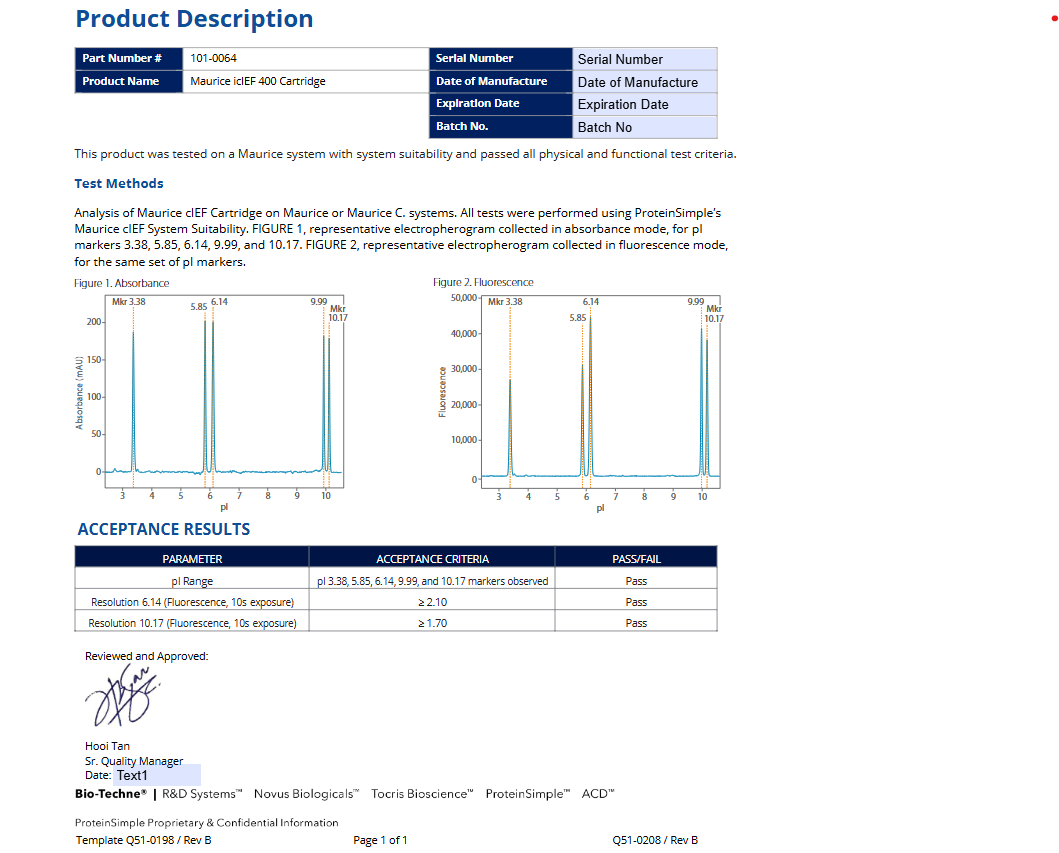
\includegraphics[width=1.0\textwidth]{template.png} % file name of your image
            
            \label{fig:example}
        \end{figure}
\end{enumerate}
Now to finish the profile creation we will have to complete the following steps.
\begin{enumerate}
  \item Inside of the profile YAML file, for each field in \textit{fields} put the appropriate data entry field. You would find the comment at the top
        of the file useful, since it lists all the possible options.
  \item Furthermore, inside of the YAML file, update the \textit{dates} entry, to indicate which of fields are dates.
  \item Lastly, make sure that you update the \textit{fonts} entry, to reflect correct fonts for fields. If no font size is specified,
        the default font size is used.
\end{enumerate}
\section{Configuration files}
When the program runs, it uses the date from multiple resources, alongside the arguments given to it. The purpose of these files is to reduce the number of
changes required in the actual code when a new configuration is necessary. In this section We want to lightly touch upon the use case of these configuration files

\subsection{Main config file (default = config.yaml at v1.0.7)}
Here is a sample printout of the configuration file alongside the explanation of each field.
\begin{lstlisting}[language=python]
run-mode1: # The mode that the program is running on
  code_map: # Path to map of code-number -> code-name
  file_perm: # Details final file permissions on created COAs
    accessibility: true
    annotate: false
    assemble: false
    copy: true
    extract: false
    form_fill: false
    modify: false
    print: true
  font: Helv # Default font of the program
  fontsize: 10 # Default fontsize of the program
  mapping_columns: # Path to where names of mapping column is stored 
  mapping_dir: # Deprecated; doesn't get used anymore
  mapping_output_dir: # List of locations where mappings will be outputted
  - ./output/ # example for mapping output
  - ./output2/ # example for mapping output
  model_dir: # Location where the models' information will be stored
  models: # List of all model profiles
  - SDS+ # example
  - cIEF 200 # example
  - ...
  pdf_output_dir: # List of locations where mapping will be outputted
  - ./output/ # example output
  prod_code_map: # Path to map of part_number -> production_code
  profile: # name for the model profile YAML file
run-mode2:
...
\end{lstlisting}
Some small notes on some of the fields listed above.
\begin{itemize}
  \item The \textit{code-map} field is a JSON file that is (number -> string)
  \item The \textit{mapping-columns} field is a JSON file with a list of strings
  \item The \textit{prod-code-map} field is an Excel file with at least 2 columns: PartNumber and ProdCode
  \item All paths can be either absolute or relative to the main executable file.
\end{itemize}

\subsection{Model Profile file}
Here is a sample printout of Maurice 200 profile YAML file printout:
\begin{lstlisting}[language=python]
dates: # List of fields that are considered dates
- Date of Manufacture
- Expiration Date
- Text1
fields: # List mapping for PDF field to Mopho data field
  Date of Manufacture: 'build_date'
  Expiration Date: 'exp_date'
  Serial Number: 'id'
  Text1: '@!TIME'
template: 046-329_CofA_Maurice_cIEF_Cartridge_090-101_RevF.pdf # Path to the template file
PN: 090-101 # Product number
color: "#B22222" # Color of the cartridge
font: # Specific fontsize for fields (optional)
  Text1: 8
\end{lstlisting}

\newpage
\section{COAT backend architecture}
\section{COAT frontend: a light overview}

\end{document}
